\documentclass[14pt]{extarticle}
% =============================================================================
% Shared Preamble for Worksheets, Homeworks, Exams & Lesson Notes
% (scripts/tex_preamble.tex)
% =============================================================================

\newif\ifdetailed
\ifdefined\setdetailed
  \setdetailed
\fi

\newif\ifwithsols
\ifdefined\setwithsols
  \setwithsols
\fi

\newif\ifwhiteblack
\ifdefined\setwhiteblack
  \setwhiteblack
\fi

% Document-class specific packages (loaded before common_preamble.tex / polyglossia)
\usepackage{fancyhdr}
\usepackage{enumitem}
\usepackage{titlesec}
\usepackage[bottom]{footmisc}
\usepackage{titling}
\usepackage{longtable} % page-breakable tables
\usepackage{float}
\usepackage[onehalfspacing]{setspace}

\ifwhiteblack
  \usepackage[a4paper, landscape, top=1.25cm, bottom=1.25cm, left=1.25cm, right=1.25cm, headheight=1.5cm, headsep=0.5cm]{geometry}
\else
  \usepackage[a4paper, top=2.4cm, bottom=2.4cm, left=2.2cm, right=2.2cm, headheight=1.4cm, headsep=0.4cm, footskip=1.0cm]{geometry}
\fi

% Shared common packages, fonts, polyglossia, callout boxes, code helpers, date & header macros
\IfFileExists{scripts/common_preamble.tex}{%
  % =============================================================================
% Shared Common Preamble (scripts/common_preamble.tex)
% Included by:
%   - scripts/tex_preamble.tex    (worksheets, homeworks, exams, lesson notes)
%   - scripts/book_preamble.tex   (two-sided Arabic book)
%   - scripts/beamer_preamble.tex (Beamer presentation slides)
% =============================================================================

\usepackage{fontspec}
\usepackage{amsmath}
\usepackage{amssymb}
\usepackage{xcolor}
\usepackage{graphicx}
\usepackage{listings}
\usepackage[most]{tcolorbox}
\usepackage{pifont}
\usepackage{minted}
\usepackage{etoolbox}
\usepackage{array}
\usepackage{booktabs}
\usepackage{tikz}
\usepackage{datetime2}

\usetikzlibrary{automata, positioning, arrows.meta, arrows, shapes.geometric, calc}

% Beamer already loads hyperref internally; load it here for article/book classes
% right before polyglossia (bidi).
\makeatletter
\@ifclassloaded{beamer}{}{%
  \usepackage{hyperref}%
  \hypersetup{hidelinks}%
  \providecommand{\LTcaptype}{table}%
}
\makeatother

% Load polyglossia (and bidi) AFTER graphics, tables, boxes, code, and hyperref
\usepackage{polyglossia}
\setmainlanguage[numerals=western]{arabic}
\setotherlanguage{english}
\newfontfamily\arabicfont[Script=Arabic]{Calibri}
\newfontfamily\arabicfontsf[Script=Arabic]{Calibri}
\newfontfamily\arabicfonttt[Script=Arabic]{Courier New}
\newfontfamily\emoji[BoldFont=*,ItalicFont=*]{Segoe UI Emoji}

% Allow slight inter-word stretch to avoid Overfull \hbox with inline \textenglish
\emergencystretch=1.5em

% -----------------------------------------------------------------------------
% Default Minted & Callout Box Definitions
% -----------------------------------------------------------------------------
\AtBeginEnvironment{minted}{\setstretch{0.95}}
\setminted{fontsize=\small, breaklines=true, vspace=2pt}

\tcbset{
  arc=2.5pt, outer arc=2.5pt,
  boxsep=1pt, left=6pt, right=6pt, top=3pt, bottom=3pt,
  toptitle=1.5pt, bottomtitle=1.5pt,
  before skip=6pt, after skip=6pt,
  fonttitle=\bfseries,
  fontupper=\setstretch{1.1}\setlength{\parskip}{2pt},
  colback=white, colframe=black, boxrule=0.6pt,
  boxcolor/.style 2 args={colback=#1, colframe=#2}
}

\newtcolorbox{boxDef}[1][]{boxcolor={blue!4!white}{blue!75!black},
  title={{\emoji📘} تعريف\ifx\\#1\\\else ~#1\fi :}}
\newtcolorbox{boxExercise}[1][]{boxcolor={cyan!4!white}{cyan!70!black},
  title={{\emoji🧩} تمرين\ifx\\#1\\\else ~#1\fi :}}
\newtcolorbox{boxExample}[1][]{boxcolor={yellow!6!white}{orange!85!black},
  title={{\emoji📝} مثال\ifx\\#1\\\else ~#1\fi :}}
\newtcolorbox{boxNote}[1][]{boxcolor={gray!7!white}{black!75},
  title={{\emoji✨} ملاحظة\ifx\\#1\\\else ~#1\fi :}}
\newtcolorbox{boxAttention}[1][]{boxcolor={magenta!5!white}{magenta!75!black},
  title={{\emoji🔔} تنبيه\ifx\\#1\\\else ~#1\fi :}}
\newtcolorbox{boxWarning}[1][]{boxcolor={red!4!white}{red!75!black},
  title={{\emoji⚡} ملاحظة هامة\ifx\\#1\\\else ~#1\fi :}}
\newtcolorbox{boxSolution}[1][]{boxcolor={green!4!white}{green!60!black},
  title={{\emoji✅} حل\ifx\\#1\\\else ~#1\fi :}}
\newtcolorbox{boxSymbol}[1][]{boxcolor={purple!4!white}{purple!70!black},
  title={{\emoji🔣} رمز\ifx\\#1\\\else ~#1\fi :}}
\newtcolorbox{boxHint}[1][]{boxcolor={teal!4!white}{teal!65!black},
  title={{\emoji💡} تلميح\ifx\\#1\\\else ~#1\fi :}}

% Compact code boxes: tighter line spacing and small vertical gaps
\tcbset{
  simplecode/.style={
    arc=2pt, outer arc=2pt,
    left=4pt, right=4pt, top=4pt, bottom=4pt,
    fontupper=\setstretch{0.95},
    before skip=6pt, after skip=6pt,
    colback=gray!5, colframe=black!50, boxrule=0.4pt
  }
}
\newenvironment{boxCode}{\begin{tcolorbox}[simplecode]}{\end{tcolorbox}}

% Code cell used inside tables (keeps code left-to-right inside RTL tables)
% Use inside a fixed-width p{...} column: \begin{pycell}\begin{minted}...\end{minted}\end{pycell}
\makeatletter
\newtcolorbox{pycell}{frame empty,colback=white,boxsep=0pt,left=2pt,right=2pt,top=2pt,bottom=2pt,width=\linewidth,before=\noindent,after=,baseline={\tcb@height-\ht\strutbox},fontupper=\setstretch{0.95}\setlength{\topsep}{0pt}\setlength{\partopsep}{0pt}\setlength{\parskip}{0pt}}
\makeatother

\newcolumntype{C}[1]{>{\centering\arraybackslash}p{#1}}

% Dotted date style (DD.MM.YYYY)
\makeatletter
\DTMnewdatestyle{dotted}{%
  \renewcommand{\DTMdisplaydate}[4]{\two@digits{##3}.\two@digits{##2}.##1}%
  \renewcommand{\DTMDisplaydate}{\DTMdisplaydate}%
}
\makeatother
\DTMsetdatestyle{dotted}

% -----------------------------------------------------------------------------
% Customizable Header / Footer Metadata
% -----------------------------------------------------------------------------
\newcommand{\headerleft}{مدرسة التسامح الشاملة}
\newcommand{\headerright}{الأستاذ محمود اغبارية}
\newcommand{\footercenter}{\thepage}

\newcommand{\setheaderleft}[1]{\renewcommand{\headerleft}{#1}}
\newcommand{\setheaderright}[1]{\renewcommand{\headerright}{#1}}
\newcommand{\setfootercenter}[1]{\renewcommand{\footercenter}{#1}}
%
}{%
  \IfFileExists{../../../scripts/common_preamble.tex}{%
    % =============================================================================
% Shared Common Preamble (scripts/common_preamble.tex)
% Included by:
%   - scripts/tex_preamble.tex    (worksheets, homeworks, exams, lesson notes)
%   - scripts/book_preamble.tex   (two-sided Arabic book)
%   - scripts/beamer_preamble.tex (Beamer presentation slides)
% =============================================================================

\usepackage{fontspec}
\usepackage{amsmath}
\usepackage{amssymb}
\usepackage{xcolor}
\usepackage{graphicx}
\usepackage{listings}
\usepackage[most]{tcolorbox}
\usepackage{pifont}
\usepackage{minted}
\usepackage{etoolbox}
\usepackage{array}
\usepackage{booktabs}
\usepackage{tikz}
\usepackage{datetime2}

\usetikzlibrary{automata, positioning, arrows.meta, arrows, shapes.geometric, calc}

% Beamer already loads hyperref internally; load it here for article/book classes
% right before polyglossia (bidi).
\makeatletter
\@ifclassloaded{beamer}{}{%
  \usepackage{hyperref}%
  \hypersetup{hidelinks}%
  \providecommand{\LTcaptype}{table}%
}
\makeatother

% Load polyglossia (and bidi) AFTER graphics, tables, boxes, code, and hyperref
\usepackage{polyglossia}
\setmainlanguage[numerals=western]{arabic}
\setotherlanguage{english}
\newfontfamily\arabicfont[Script=Arabic]{Calibri}
\newfontfamily\arabicfontsf[Script=Arabic]{Calibri}
\newfontfamily\arabicfonttt[Script=Arabic]{Courier New}
\newfontfamily\emoji[BoldFont=*,ItalicFont=*]{Segoe UI Emoji}

% Allow slight inter-word stretch to avoid Overfull \hbox with inline \textenglish
\emergencystretch=1.5em

% -----------------------------------------------------------------------------
% Default Minted & Callout Box Definitions
% -----------------------------------------------------------------------------
\AtBeginEnvironment{minted}{\setstretch{0.95}}
\setminted{fontsize=\small, breaklines=true, vspace=2pt}

\tcbset{
  arc=2.5pt, outer arc=2.5pt,
  boxsep=1pt, left=6pt, right=6pt, top=3pt, bottom=3pt,
  toptitle=1.5pt, bottomtitle=1.5pt,
  before skip=6pt, after skip=6pt,
  fonttitle=\bfseries,
  fontupper=\setstretch{1.1}\setlength{\parskip}{2pt},
  colback=white, colframe=black, boxrule=0.6pt,
  boxcolor/.style 2 args={colback=#1, colframe=#2}
}

\newtcolorbox{boxDef}[1][]{boxcolor={blue!4!white}{blue!75!black},
  title={{\emoji📘} تعريف\ifx\\#1\\\else ~#1\fi :}}
\newtcolorbox{boxExercise}[1][]{boxcolor={cyan!4!white}{cyan!70!black},
  title={{\emoji🧩} تمرين\ifx\\#1\\\else ~#1\fi :}}
\newtcolorbox{boxExample}[1][]{boxcolor={yellow!6!white}{orange!85!black},
  title={{\emoji📝} مثال\ifx\\#1\\\else ~#1\fi :}}
\newtcolorbox{boxNote}[1][]{boxcolor={gray!7!white}{black!75},
  title={{\emoji✨} ملاحظة\ifx\\#1\\\else ~#1\fi :}}
\newtcolorbox{boxAttention}[1][]{boxcolor={magenta!5!white}{magenta!75!black},
  title={{\emoji🔔} تنبيه\ifx\\#1\\\else ~#1\fi :}}
\newtcolorbox{boxWarning}[1][]{boxcolor={red!4!white}{red!75!black},
  title={{\emoji⚡} ملاحظة هامة\ifx\\#1\\\else ~#1\fi :}}
\newtcolorbox{boxSolution}[1][]{boxcolor={green!4!white}{green!60!black},
  title={{\emoji✅} حل\ifx\\#1\\\else ~#1\fi :}}
\newtcolorbox{boxSymbol}[1][]{boxcolor={purple!4!white}{purple!70!black},
  title={{\emoji🔣} رمز\ifx\\#1\\\else ~#1\fi :}}
\newtcolorbox{boxHint}[1][]{boxcolor={teal!4!white}{teal!65!black},
  title={{\emoji💡} تلميح\ifx\\#1\\\else ~#1\fi :}}

% Compact code boxes: tighter line spacing and small vertical gaps
\tcbset{
  simplecode/.style={
    arc=2pt, outer arc=2pt,
    left=4pt, right=4pt, top=4pt, bottom=4pt,
    fontupper=\setstretch{0.95},
    before skip=6pt, after skip=6pt,
    colback=gray!5, colframe=black!50, boxrule=0.4pt
  }
}
\newenvironment{boxCode}{\begin{tcolorbox}[simplecode]}{\end{tcolorbox}}

% Code cell used inside tables (keeps code left-to-right inside RTL tables)
% Use inside a fixed-width p{...} column: \begin{pycell}\begin{minted}...\end{minted}\end{pycell}
\makeatletter
\newtcolorbox{pycell}{frame empty,colback=white,boxsep=0pt,left=2pt,right=2pt,top=2pt,bottom=2pt,width=\linewidth,before=\noindent,after=,baseline={\tcb@height-\ht\strutbox},fontupper=\setstretch{0.95}\setlength{\topsep}{0pt}\setlength{\partopsep}{0pt}\setlength{\parskip}{0pt}}
\makeatother

\newcolumntype{C}[1]{>{\centering\arraybackslash}p{#1}}

% Dotted date style (DD.MM.YYYY)
\makeatletter
\DTMnewdatestyle{dotted}{%
  \renewcommand{\DTMdisplaydate}[4]{\two@digits{##3}.\two@digits{##2}.##1}%
  \renewcommand{\DTMDisplaydate}{\DTMdisplaydate}%
}
\makeatother
\DTMsetdatestyle{dotted}

% -----------------------------------------------------------------------------
% Customizable Header / Footer Metadata
% -----------------------------------------------------------------------------
\newcommand{\headerleft}{مدرسة التسامح الشاملة}
\newcommand{\headerright}{الأستاذ محمود اغبارية}
\newcommand{\footercenter}{\thepage}

\newcommand{\setheaderleft}[1]{\renewcommand{\headerleft}{#1}}
\newcommand{\setheaderright}[1]{\renewcommand{\headerright}{#1}}
\newcommand{\setfootercenter}[1]{\renewcommand{\footercenter}{#1}}
%
  }{%
    \input{../../scripts/common_preamble.tex}%
  }%
}

\pagestyle{fancy}

% Prevent widow/orphan lines
\widowpenalty=10000
\clubpenalty=10000

% Compact section headings and default list spacing so pages do not waste vertical space
\titlespacing*{\section}{0pt}{1.4ex plus 0.4ex minus 0.2ex}{0.7ex plus 0.2ex}
\titlespacing*{\subsection}{0pt}{1.1ex plus 0.3ex minus 0.2ex}{0.5ex plus 0.1ex}
\titlespacing*{\subsubsection}{0pt}{0.9ex plus 0.2ex minus 0.1ex}{0.4ex plus 0.1ex}
\setlist{topsep=4pt, partopsep=0pt, parsep=2pt, itemsep=4pt}

\gappto\captionsarabic{\renewcommand{\contentsname}{جدول المحتويات}}

% Legacy listings settings
\lstset{
  language=[Sharp]C,
  numbers=left,
  stepnumber=1,
  numbersep=8pt,
  frame=single,
  basicstyle=\ttfamily\small
}
\ifwhiteblack
  \lstset{
    keywordstyle=\bfseries,
    stringstyle=\ttfamily,
    commentstyle=\itshape
  }
\else
  \lstset{
    keywordstyle=\color{blue},
    stringstyle=\color{red},
    commentstyle=\color{green!50!black}
  }
\fi

% White-and-black landscape presentation mode overrides
\ifwhiteblack
  \AtBeginDocument{
    \LARGE
    \usemintedstyle{bw}
  }
  \setminted{vspace=2pt}
  \tcbset{
    colback=white, colframe=black, boxrule=1pt,
    boxcolor/.style 2 args={colback=white, colframe=black},
    simplecode/.append style={colback=white, colframe=black, boxrule=1pt}
  }
\fi

% Default to empty author to avoid "LaTeX Warning: No \author given" when omitted
\author{}

% Compact title block
\makeatletter
\renewcommand{\@maketitle}{%
  \begin{center}%
    {\ifwhiteblack\Huge\else\LARGE\fi \bfseries \@title \par}%
    \ifdefempty{\@author}{}{%
      \vskip 0.15em%
      {\large \@author \par}%
    }%
    {\small \hfill \textenglish{\DTMtoday} \par}%
  \end{center}%
  \vspace{-0.3cm}%
}
\makeatother

\apptocmd{\maketitle}{\thispagestyle{fancy}}{}{}

% Apply page headers and footer (using \headerleft, \headerright, \footercenter from common_preamble.tex)
\newcommand{\applyfancyheaders}{%
  \fancyhf{}%
  \fancyhead[L]{\textarabic{\headerleft}}%
  \fancyhead[R]{\textarabic{\headerright}}%
  \fancyfoot[C]{\textarabic{\footercenter}}%
}

\fancypagestyle{plain}{\applyfancyheaders}
\applyfancyheaders

\setcounter{tocdepth}{3} % only section, subsection, and subsubsection in TOC

\newcommand{\importpdfpage}[2]{%
    \newgeometry{left=0cm,right=0cm,top=0cm,bottom=0cm}
    \thispagestyle{empty}
    \includegraphics[page=#2,width=0.95\paperwidth,height=0.95\paperheight,keepaspectratio]{#1}
    \restoregeometry
}

\newcommand{\insertFullImg}[1]{%
    \noindent
    \makebox[\textwidth][c]{
        \includegraphics[width=0.9\paperwidth,keepaspectratio]{#1}%
    }%
}%


\usetikzlibrary{arrows.meta, positioning, shapes.geometric, fit, backgrounds}

\title{ملخص: كيف يحدّد الحاسوب أيّ عملية تُستدعى؟ (زمن التجميع مقابل زمن التشغيل)}

\begin{document}

\maketitle
\thispagestyle{fancy}

\begin{boxDef}[- الفكرة المركزية]
عندما يرى الحاسوب أمر استدعاء عملية مثل \textenglish{x.Foo(y)} في لغة \textenglish{C\#}، فإنّه لا يختار العملية دفعةً واحدة، بل يمرّ بـ\textbf{مرحلتين منفصلتين}: مرحلة \textbf{زمن التجميع} (قبل تشغيل البرنامج)، ثمّ مرحلة \textbf{زمن التشغيل} (أثناء تنفيذ البرنامج فعليًا).
\end{boxDef}

% ==============================================================
\section*{أوّلًا: القاعدة الذهبية بخطوتين}
% ==============================================================

\begin{enumerate}[itemsep=0.8em]
    \item \textbf{في زمن التجميع (مسح الأوامر):} ينظر المُجمّع فقط إلى \textbf{النمط الساكن} للمتغيّر الذي نُفعّل عليه العملية، وإلى \textbf{النمط الساكن للمُعطيات} المُمرّرة داخل الأقواس (ولا يعرف شيئًا عن الكائن الفعلي في الذاكرة). يبحث عن أنسب عملية مطابقة:
    \begin{itemize}
        \item إذا لم يجد عملية مناسبة $\leftarrow$ ينتج \textbf{خطأ في التجميع}.
        \item إذا وجدها $\leftarrow$ يثبّت توقيع هذه العملية كهدف للاستدعاء.
    \end{itemize}
    \filbreak
    \item \textbf{في زمن التشغيل (تنفيذ الأوامر):} ينظر الحاسوب إلى \textbf{النمط الفعلي} للكائن الموجود في الذاكرة:
    \begin{itemize}
        \item إذا كانت العملية التي اختيرت في الخطوة ($1$) من نوع \textenglish{virtual} (أو \textenglish{override} أو \textenglish{abstract}) $\leftarrow$ ينزل إلى \textbf{آخر \textenglish{override}} لهذه العملية في الكائن الفعلي وينفّذه.
        \item وإلّا (ليست \textenglish{virtual}، أو كانت عملية ساكنة \textenglish{static}) $\leftarrow$ ينفّذ نفس العملية التي اختيرت في الخطوة ($1$) مباشرةً.
    \end{itemize}
    \filbreak
\end{enumerate}

\begin{center}
\begin{english}
\begin{tikzpicture}[
    node distance=0.85cm and 1.1cm,
    box/.style={rectangle, rounded corners=6pt, draw=blue!65!black, fill=blue!6, thick, text width=6.2cm, align=center, inner sep=7pt},
    runbox/.style={rectangle, rounded corners=6pt, draw=teal!70!black, fill=teal!7, thick, text width=5.6cm, align=center, inner sep=7pt},
    errbox/.style={rectangle, rounded corners=6pt, draw=red!70!black, fill=red!7, thick, text width=4.0cm, align=center, inner sep=6pt},
    dec/.style={rectangle, rounded corners=4pt, draw=orange!80!black, fill=orange!10, thick, text width=5.6cm, align=center, inner sep=6pt},
    arr/.style={-{Stealth[length=3mm]}, thick, draw=black!75}
]
    \node[box] (step1) {\textbf{\textarabic{الخطوة 1: زمن التجميع}}\\[2pt]
        \small\textarabic{فحص النمط الساكن للمتغيّر وللمُعطيات}\\
        \small\textarabic{واختيار توقيع العملية الأنسب}};

    \node[errbox, right=1.2cm of step1] (err) {\textbf{\textarabic{خطأ في التجميع}}\\[2pt]
        \small\textarabic{لم تُوجَد عملية مطابقة}};

    \node[dec, below=0.9cm of step1] (check) {\textbf{\textarabic{الخطوة 2: زمن التشغيل}}\\[2pt]
        \small\textarabic{هل العملية المختارة \textenglish{virtual} / \textenglish{override}؟}};

    \node[runbox, below left=0.95cm and -1.8cm of check] (yes) {\textbf{\textarabic{نعم (ربط ديناميكي)}}\\[2pt]
        \small\textarabic{استدعاء \textbf{آخر \textenglish{override}} في النمط الفعلي للكائن}};

    \node[runbox, draw=purple!70!black, fill=purple!6, below right=0.95cm and -1.8cm of check] (no) {\textbf{\textarabic{لا (ربط ساكن)}}\\[2pt]
        \small\textarabic{تنفيذ نفس العملية المختارة في زمن التجميع مباشرةً}};

    \draw[arr] (step1.east) -- node[above, font=\small]{\textarabic{لا توجد}} (err.west);
    \draw[arr] (step1.south) -- node[right, font=\small]{\textarabic{وُجِدت عملية}} (check.north);
    \draw[arr] (check.west) -| node[pos=0.25, above, font=\small]{\textarabic{نعم}} (yes.north);
    \draw[arr] (check.east) -| node[pos=0.25, above, font=\small]{\textarabic{لا}} (no.north);
\end{tikzpicture}
\end{english}
\end{center}

\begin{boxAttention}[- نقطتان مهمّتان]
\begin{itemize}
    \item \textbf{العملية \textenglish{override} تبقى \textenglish{virtual} تلقائيًا:} إذا ورثت الفئة $C$ من $B$، وكانت العملية في $B$ تحمل \textenglish{override}، فإنّها تظلّ قابلة للربط الديناميكي نحو $C$.
    \item \textbf{استدعاء \textenglish{base.Foo()}:} يتجاوز الخطوة ($2$) وينفّذ مباشرةً نسخة الفئة الأب.
\end{itemize}
\end{boxAttention}

% ==============================================================
\clearpage
\section*{ثانيًا: تطبيق القاعدة على ثلاث حالات أساسية}
% ==============================================================

\filbreak
\subsection*{الحالة الأولى: التحميل الزائد — النمط الساكن للمُعطى هو الحاسم}
في التحميل الزائد توجد عمليتان بنفس الاسم ولكن بمعطيات مختلفة. اختيار أيّ منهما يُحسم \textbf{بالكامل في زمن التجميع} حسب النمط الساكن للمُعطى المُمرّر:

\begin{boxCode}
\begin{english}
\begin{minted}{csharp}
public class A { }
public class B : A { }

public static void Foo(A x) { Console.WriteLine("Foo(A)"); }
public static void Foo(B x) { Console.WriteLine("Foo(B)"); }

// In Main:
A a = new A();
B b = new B();
A c = b;        // Static type: A, Runtime type: B
Foo(a);         // Output: Foo(A)
Foo(b);         // Output: Foo(B)
Foo(c);         // Output: Foo(A)  <-- static type of c is A!
\end{minted}
\end{english}
\end{boxCode}

\textbf{لماذا طبع \textenglish{Foo(c)} النتيجة \textenglish{Foo(A)}؟}
لأنّ النمط الساكن للمتغيّر $c$ هو $A$، ففي \textbf{زمن التجميع} يختار الحاسوب العملية \textenglish{Foo(A)}. وبما أنّ \textenglish{Foo} ليست \textenglish{virtual} (بل عملية ساكنة)، فلا يتغيّر القرار في زمن التشغيل.

\filbreak
\subsection*{الحالة الثانية: غياب \textenglish{virtual} / \textenglish{override} مقابل وجودهما}
لنقارن بين كتابة عملية \textenglish{Print} في الفئتين $A$ و$B$ \textbf{بدون} \textenglish{virtual}/\textenglish{override} مقابل كتابتها \textbf{مع} \textenglish{virtual}/\textenglish{override}:

\begin{boxCode}
\begin{english}
\begin{minted}{csharp}
// Case 1: WITHOUT virtual / override
public class A
{
    public void Print() { Console.WriteLine("A"); }
}
public class B : A
{
    public void Print() { Console.WriteLine("B"); }
}

// Case 2: WITH virtual / override
public class A2
{
    public virtual void Print() { Console.WriteLine("A"); }
}
public class B2 : A2
{
    public override void Print() { Console.WriteLine("B"); }
}
\end{minted}
\end{english}
\end{boxCode}

\begin{center}
\begin{english}
\begin{tikzpicture}[
    var/.style={rectangle, draw=blue!70!black, fill=blue!8, thick, minimum width=2.2cm, minimum height=0.9cm, align=center},
    partA/.style={rectangle, draw=black!75, fill=gray!10, thick, minimum width=3.9cm, minimum height=0.9cm, align=center, font=\small},
    partB/.style={rectangle, draw=teal!75!black, fill=teal!10, thick, minimum width=3.9cm, minimum height=0.9cm, align=center, font=\small},
    arr/.style={-{Stealth[length=2.8mm]}, thick}
]
    \node[var] (c) {\texttt{A c}\\[-1pt]\scriptsize\textarabic{النمط الساكن: \textenglish{A}}};

    \node[partA, right=1.1cm of c, yshift=0.45cm] (objA) {\texttt{A.Print()} $\rightarrow$ \texttt{"A"}};
    \node[partB, below=0pt of objA] (objB) {\texttt{B.Print()} $\rightarrow$ \texttt{"B"}};

    \begin{scope}[on background layer]
        \node[draw=teal!80!black, dashed, rounded corners=4pt, fit=(objA)(objB), inner sep=5pt,
              label={[teal!80!black, font=\small]above:{\textarabic{الكائن الفعلي في الذاكرة: \textenglish{\texttt{new B()}}}}}] (heap) {};
    \end{scope}

    \draw[arr, blue!75!black] (c.east) -- node[above, font=\scriptsize]{\textarabic{مؤشر}} (heap.west);

    % Right side arrows explaining Case 1 vs Case 2
    \node[right=0.9cm of objA, align=right, font=\small, text=purple!80!black] (lbl1)
        {\textarabic{بدون \textenglish{virtual}: يتوقف هنا $\leftarrow$ يطبع \textenglish{"A"}}};
    \node[right=0.9cm of objB, align=right, font=\small, text=teal!80!black] (lbl2)
        {\textarabic{مع \textenglish{virtual}/\textenglish{override}: ينزل هنا $\leftarrow$ يطبع \textenglish{"B"}}};

    \draw[arr, purple!80!black] (objA.east) -- (lbl1.west);
    \draw[arr, teal!80!black, dashed] (objA.south east) to[bend right=35] (objB.north east);
    \draw[arr, teal!80!black] (objB.east) -- (lbl2.west);
\end{tikzpicture}
\end{english}
\end{center}

\begin{boxNote}[- ملاحظة للبجروت]
في أسئلة البجروت، كلّما أراد واضع الامتحان إعادة تعريف عملية في الابن فإنّه يكتب \textenglish{virtual} في الأب و\textenglish{override} في الابن؛ أمّا فهم الفرق أعلاه فيوضّح لماذا لا يعمل تعدّد الأشكال بدونهما في لغة \textenglish{C\#}.
\end{boxNote}

% ==============================================================
\clearpage
\section*{ثالثًا: مثال شامل على نمط أسئلة البجروت}
% ==============================================================

في أسئلة البجروت الحديثة (مثل صيف $2019$، $2025$، $2026$) يُدمَج \textbf{التحميل الزائد} مع \textbf{إعادة التعريف} في هرمية من ثلاث فئات. تأمّل الفئات التالية:

\begin{boxCode}
\begin{english}
\begin{minted}{csharp}
public class A
{
    public virtual void Work(B other) { Console.WriteLine("A.Work(B)"); }
}
public class B : A
{
    public override void Work(B other) { Console.WriteLine("B.Work(B)"); }
    public void Work(A other)          { Console.WriteLine("B.Work(A)"); }
}
public class C : B
{
    public override void Work(B other) { Console.WriteLine("C.Work(B)"); }
    public void Work(C other)          { Console.WriteLine("C.Work(C)"); }
}
\end{minted}
\end{english}
\end{boxCode}

\begin{center}
\begin{english}
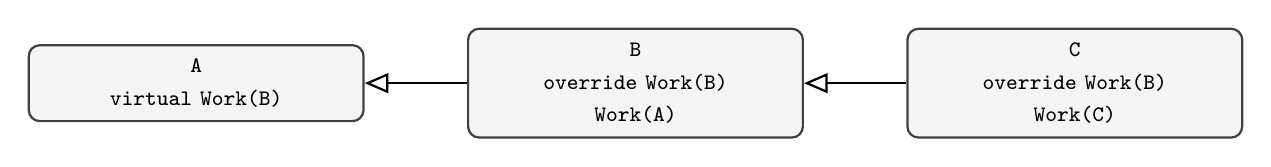
\begin{tikzpicture}[
    cls/.style={rectangle, rounded corners=4pt, draw=black!75, fill=gray!8, thick, text width=3.9cm, align=center, inner sep=5pt, font=\footnotesize},
    inh/.style={-{Triangle[open, length=3mm, width=2.5mm]}, thick}
]
    \node[cls] (A) {\textbf{\texttt{A}}\\\texttt{virtual Work(B)}};
    \node[cls, right=1.3cm of A] (B) {\textbf{\texttt{B}}\\\texttt{override Work(B)}\\\texttt{Work(A)}};
    \node[cls, right=1.3cm of B] (C) {\textbf{\texttt{C}}\\\texttt{override Work(B)}\\\texttt{Work(C)}};

    \draw[inh] (B.west) -- (A.east);
    \draw[inh] (C.west) -- (B.east);
\end{tikzpicture}
\end{english}
\end{center}

افترض الآن أنّنا أنشأنا في \textenglish{Main} الكائنات التالية:

\begin{boxCode}
\begin{english}
\begin{minted}{csharp}
A ab = new B();   // Static: A, Runtime: B
A ac = new C();   // Static: A, Runtime: C
B bc = new C();   // Static: B, Runtime: C
C c  = new C();   // Static: C, Runtime: C
\end{minted}
\end{english}
\end{boxCode}

تتبّع كل استدعاء باستخدام \textbf{الخطوتين} بدقّة:

{\renewcommand{\arraystretch}{1.25}
\small
\begin{longtable}{|>{\raggedright\arraybackslash}p{0.21\textwidth}|>{\raggedleft\arraybackslash}p{0.26\textwidth}|>{\raggedleft\arraybackslash}p{0.25\textwidth}|>{\raggedright\arraybackslash}p{0.15\textwidth}|}
\hline
\textbf{أمر الاستدعاء} & \textbf{الخطوة $1$: زمن التجميع (النمط الساكن)} & \textbf{الخطوة $2$: زمن التشغيل (النمط الفعلي)} & \textbf{المُخرَج} \\
\hline
\endhead

\textenglish{ac.Work(bc);} &
الساكن لـ \textenglish{ac} هو $A$ ولـ \textenglish{bc} هو $B$ $\leftarrow$ يختار \textenglish{A.Work(B)} (وهي \textenglish{virtual}). &
الفعلي لـ \textenglish{ac} هو $C$ $\leftarrow$ ينزل إلى آخر \textenglish{override} في $C$. &
\textenglish{C.Work(B)} \\
\hline

\textenglish{c.Work(ac);} &
الساكن لـ $c$ هو $C$ ولـ \textenglish{ac} هو $A$ $\leftarrow$ أنسب عملية هي \textenglish{B.Work(A)} الموروثة (ليست \textenglish{virtual}). &
ليست \textenglish{virtual} $\leftarrow$ تُنفّذ \textenglish{B.Work(A)} مباشرةً. &
\textenglish{B.Work(A)} \\
\hline

\textenglish{((B)ab).Work(ab);} &
الساكن بعد التحويل هو $B$ والساكن لـ \textenglish{ab} هو $A$ $\leftarrow$ يختار \textenglish{B.Work(A)} (ليست \textenglish{virtual}). &
التحويل سليم (الفعلي $B$)، والعملية ليست \textenglish{virtual} $\leftarrow$ تُنفّذ مباشرةً. &
\textenglish{B.Work(A)} \\
\hline

\textenglish{((C)bc).Work(c);} &
الساكن بعد التحويل هو $C$ ولـ $c$ هو $C$ $\leftarrow$ يختار \textenglish{C.Work(C)} (ليست \textenglish{virtual}). &
التحويل سليم (الفعلي $C$) $\leftarrow$ تُنفّذ \textenglish{C.Work(C)} مباشرةً. &
\textenglish{C.Work(C)} \\
\hline

\textenglish{ab.Work(ac);} &
الساكن لـ \textenglish{ab} هو $A$، وفي $A$ توجد فقط \textenglish{Work(B)} بينما الساكن لـ \textenglish{ac} هو $A$! &
لا يصل إلى زمن التشغيل. &
\textarabic{\textbf{خطأ تجميع}} \\
\hline
\end{longtable}}

\begin{boxWarning}[- الفخّ الأكثر تكرارًا في البجروت]
في السطر \textenglish{c.Work(ac);} ينخدع كثير من الطلاب ويظنّون أنّ \textenglish{C.Work(C)} ستُستدعى لأنّ الكائن الفعلي لـ \textenglish{ac} هو $C$. تذكّروا دائمًا: \textbf{النمط الفعلي يؤثّر فقط على الكائن الذي قبل النقطة} (وذلك فقط إذا كانت العملية المختارة \textenglish{virtual} أو \textenglish{override})، أمّا \textbf{المُعطى داخل الأقواس فيُحسَم دائمًا حسب نمطه الساكن في زمن التجميع!}
\end{boxWarning}

\vspace{1cm}
\begin{flushleft}
أرجو لكم وقتًا ممتعًا.

الأستاذ محمود اغبارية.
\end{flushleft}

\end{document}
